\setcounter{secnumdepth}{-1} % Убираем нумерацию секций

\section{Введение}

В данной лабораторной работе рассматриваются методы анализа 
устойчивости нелинейных динамических систем с использованием 
функций Ляпунова, а также синтез стабилизирующих регуляторов 
на основе линейных матричных неравенств (LMI).

\section{1. Анализ устойчивости с использованием кандидата квадратичной функции Ляпунова}

Для каждой из следующих систем используем кандидат квадратичной 
функции Ляпунова $V(x) = x_1^2 + x_2^2$ (для скалярной системы $V(x) = x^2$).

\subsection*{Система 1}

Рассмотрим систему:
\begin{align*}
\dot{x}_1 &= -x_1 + x_1 x_2 \\
\dot{x}_2 &= -2x_2
\end{align*}

Найдем производную функции Ляпунова $V(x) = x_1^2 + x_2^2$:
\begin{align*}
\dot{V} &= 2x_1 \dot{x}_1 + 2x_2 \dot{x}_2 \\
&= 2x_1(-x_1 + x_1 x_2) + 2x_2(-2x_2) \\
&= -2x_1^2 + 2x_1^2 x_2 - 4x_2^2 \\
&= -2x_1^2 (1 - x_2) - 4x_2^2
\end{align*}

\textbf{Анализ устойчивости:}

При $x_2 < 1$: $\dot{V} < 0$. Следовательно, система асимптотически
устойчива в окрестности начала координат, но не является глобально устойчивой.

\subsection{Система 2}

Рассмотрим систему:
\begin{align*}
\dot{x}_1 &= -x_2 - x_1(1 - x_1^2 - x_2^2) \\
\dot{x}_2 &= x_1 - x_2(1 - x_1^2 - x_2^2)
\end{align*}

Найдем производную функции Ляпунова $V(x) = x_1^2 + x_2^2$:
\begin{align*}
\dot{V} &= 2x_1 \dot{x}_1 + 2x_2 \dot{x}_2 \\
&= 2x_1\left(-x_2 - x_1(1 - x_1^2 - x_2^2)\right) + 2x_2\left(x_1 - x_2(1 - x_1^2 - x_2^2)\right) \\
&= -2x_1 x_2 - 2x_1^2(1 - x_1^2 - x_2^2) + 2x_1 x_2 - 2x_2^2(1 - x_1^2 - x_2^2) \\
&= -2(x_1^2 + x_2^2)(1 - x_1^2 - x_2^2)
\end{align*}

\textbf{Анализ устойчивости:}

При $x_1^2 + x_2^2 < 1$: $\dot{V} < 0$. Следовательно, область устойчивости 
ограничена единичным кругом, поэтому система локально асимптотически устойчива, 
но не является глобально устойчивой.

\subsection{Система 3}

Рассмотрим систему:
\begin{align*}
\dot{x}_1 &= x_2(1 - x_1^2) - 2x_1 \\
\dot{x}_2 &= -(x_1 + x_2)(1 - x_1^2)
\end{align*}

Найдем производную функции Ляпунова $V(x) = x_1^2 + x_2^2$:
\begin{align*}
\dot{V} &= 2x_1\left(x_2(1 - x_1^2) - 2x_1\right) + 2x_2\left(-(x_1 + x_2)(1 - x_1^2)\right) \\
&= 2x_1 x_2(1 - x_1^2) - 4x_1^2 - 2x_1 x_2(1 - x_1^2) - 2x_2^2(1 - x_1^2) \\
&= -4x_1^2 - 2x_2^2(1 - x_1^2)
\end{align*}

\textbf{Анализ устойчивости:}

При $x_1 < 1$: $\dot{V} < 0$. Следовательно, система асимптотически
устойчива в окрестности начала координат, но не является глобально устойчивой.

\subsection*{Система 4}

Рассмотрим систему:
\begin{align*}
\dot{x}_1 &= -3x_1 - x_2 \\
\dot{x}_2 &= 2x_1 - x_2^3
\end{align*}

Найдем производную функции Ляпунова $V(x) = x_1^2 + x_2^2$:
\begin{align*}
\dot{V} &= 2x_1(-3x_1 - x_2) + 2x_2(2x_1 - x_2^3) \\
&= -6x_1^2 - 2x_1 x_2 + 4x_1 x_2 - 2x_2^4 \\
&= -6x_1^2 + 2x_1 x_2 - 2x_2^4
\end{align*}

\textbf{Анализ устойчивости:}

При $2x_1 x_2 < 6x_1^2 + 2x_2^4$: $\dot{V} < 0$.
Неравенство выполняется для любых $x_1$ и $x_1$.
Следовательно, система глобально асимптотически устойчива.

\subsection*{Система 5}

Рассмотрим скалярную систему:
\begin{align*}
\dot{x} = -\arctan(x)
\end{align*}

Найдем производную функции Ляпунова $V(x) = x^2$:
\begin{align*}
\dot{V} &= 2x \dot{x} = 2x(-\arctan(x)) = -2x\arctan(x)
\end{align*}

\textbf{Анализ устойчивости:}

Так как $\arctan(-x) = -\arctan(x)$, то $\dot{V} < 0$ везде, кроме 0. 
Следовательно, система глобально асимптотически устойчива.


\section{2. Условия асимптотической устойчивости скалярной системы}

Рассмотрим скалярную систему:
\begin{align*}
\dot{x} = ax^p + h(x)
\end{align*}
где $p$ — натуральное число, а $h(x)$ удовлетворяет условию $|h(x)| \leq k|x|^{p+1}$ в некоторой окрестности точки начала координат.

Требуется определить условия, при которых система асимптотически устойчива.

Выберем функцию Ляпунова $V=\frac{1}{2}x^2$. Возьмем производную:
\begin{align*}
\dot{V} = x\dot{x} = x(ax^p + h(x)) = ax^{p+1} + xh(x)
\end{align*}

Учитывая условие задания 
\begin{align*}
|xh(x)| \le |x| \dot k|x|^{p+1} = k|x|^{p+2}
\end{align*}

получим 
\begin{align*}
& \dot{V} = ax^{p+1} + xh(x) \le ax^{p+1} + k|x|^{p+2} \\
& |xh(x)| \leq k|x|^{p+2} \ll |ax^{p+1}| - \text{в малой окрестности начала координат}
\end{align*}

\subsection{Случай 1: $p$ — нечетное число}

При нечетном $p$ имеем $x^{p+1} \geq 0$ для всех $x$.

\begin{itemize}
\item Если $a < 0$, то $ax^{p+1} \leq 0$ для всех $x$.
Тогда $\dot{V} < 0$ $\Rightarrow$ система асимптотически устойчива.
\item Если $a > 0$, то $ax^{p+1} \geq 0$ для всех $x$.
Тогда $\dot{V} > 0$ $\Rightarrow$ система неустойчива.
\end{itemize}

\subsection{Случай 2: $p$ — четное число}

При четном $p$ имеем $x^{p+1}$ имеет тот же знак, что и $x$.

\begin{itemize}
\item Если $a < 0$, то $ax^{p+1} < 0$ при $x > 0$ и $ax^{p+1} > 0$ при $x < 0$.
Тогда $\dot{V} < 0$ при $x > 0$ и $\dot{V} > 0$ при $x < 0$ $\Rightarrow$ система неустойчива.
\item Если $a > 0$, то $ax^{p+1} > 0$ при $x > 0$ и $ax^{p+1} < 0$ при $x < 0$.
Тогда $\dot{V} > 0$ при $x > 0$ и $\dot{V} < 0$ при $x < 0$ $\Rightarrow$ система неустойчива.
\end{itemize}

\subsection{Случай 3: $a = 0$}

При $a = 0$ имеем $\dot{x} = h(x)$. Таким образом, устойчивость системы зависит от конкретного вида $h(x)$.

\subsection{Условие асимптотической устойчивости:}
\begin{itemize}
\item $|h(x)| \leq k|x|^{p+1}$ - в малой окрестности начала координат;
\item $p$ - нечетное число;
\item $a < 0$.
\end{itemize}

\section*{Задача 3. Синтез линейного регулятора через LMI}

На основе применения LMI построим линейный регулятор, стабилизирующий систему экспоненциально со степенью 2:

\begin{align}
\dot{x}_1 &= x_2 \\
\dot{x}_2 &= 2x_1 + u
\end{align}

\subsection*{Постановка задачи}

Требуется найти матрицу обратной связи $K$ такую, что замкнутая система $\dot{x} = (A + BK)x$ имеет экспоненциальную устойчивость степени 2, то есть:

\begin{equation}
\|x(t)\| \leq M\|x(0)\|e^{-2t}
\end{equation}

для некоторого $M > 0$ и всех $t \geq 0$.

Матрицы системы:
\begin{align}
A &= \begin{pmatrix} 0 & 1 \\ 2 & 0 \end{pmatrix}, \quad
B &= \begin{pmatrix} 0 \\ 1 \end{pmatrix}
\end{align}

\subsection*{Анализ управляемости}

Матрица управляемости:
\begin{equation}
C = [B, AB] = \begin{pmatrix} 0 & 1 \\ 1 & 0 \end{pmatrix}
\end{equation}

Ранг матрицы управляемости равен 2, поэтому система полностью управляема.

Собственные значения разомкнутой системы: $\lambda = \pm\sqrt{2} \approx \pm 1.414$, что означает неустойчивость.

\subsection*{Синтез регулятора}

\subsubsection*{Метод размещения полюсов}

Для обеспечения экспоненциальной устойчивости степени 2 выберем желаемые полюса: $\lambda_1 = -3$, $\lambda_2 = -4$.

Желаемый характеристический полином:
\begin{equation}
(s + 3)(s + 4) = s^2 + 7s + 12
\end{equation}

Для системы с матрицами $A$, $B$ находим $K$ такой, что:
\begin{equation}
\det(sI - (A + BK)) = s^2 + 7s + 12
\end{equation}

Матрица замкнутой системы:
\begin{equation}
A + BK = \begin{pmatrix} 0 & 1 \\ 2 + k_1 & k_2 \end{pmatrix}
\end{equation}

Характеристический полином:
\begin{equation}
\det(sI - (A + BK)) = s^2 - k_2s - (2 + k_1)
\end{equation}

Приравнивая коэффициенты:
\begin{align}
-k_2 &= 7 \Rightarrow k_2 = -7 \\
-(2 + k_1) &= 12 \Rightarrow k_1 = -14
\end{align}

Получаем матрицу обратной связи:
\begin{equation}
K = \begin{pmatrix} -14 & -7 \end{pmatrix}
\end{equation}

\subsubsection*{Проверка собственных значений}

Собственные значения замкнутой системы:
\begin{equation}
\lambda = -3, \quad \lambda = -4
\end{equation}

Максимальная вещественная часть: $\max(\text{Re}(\lambda)) = -3 < -2$, что обеспечивает требуемую экспоненциальную устойчивость степени 2.

\subsection*{Моделирование замкнутой системы}

\begin{figure}[H]
\centering
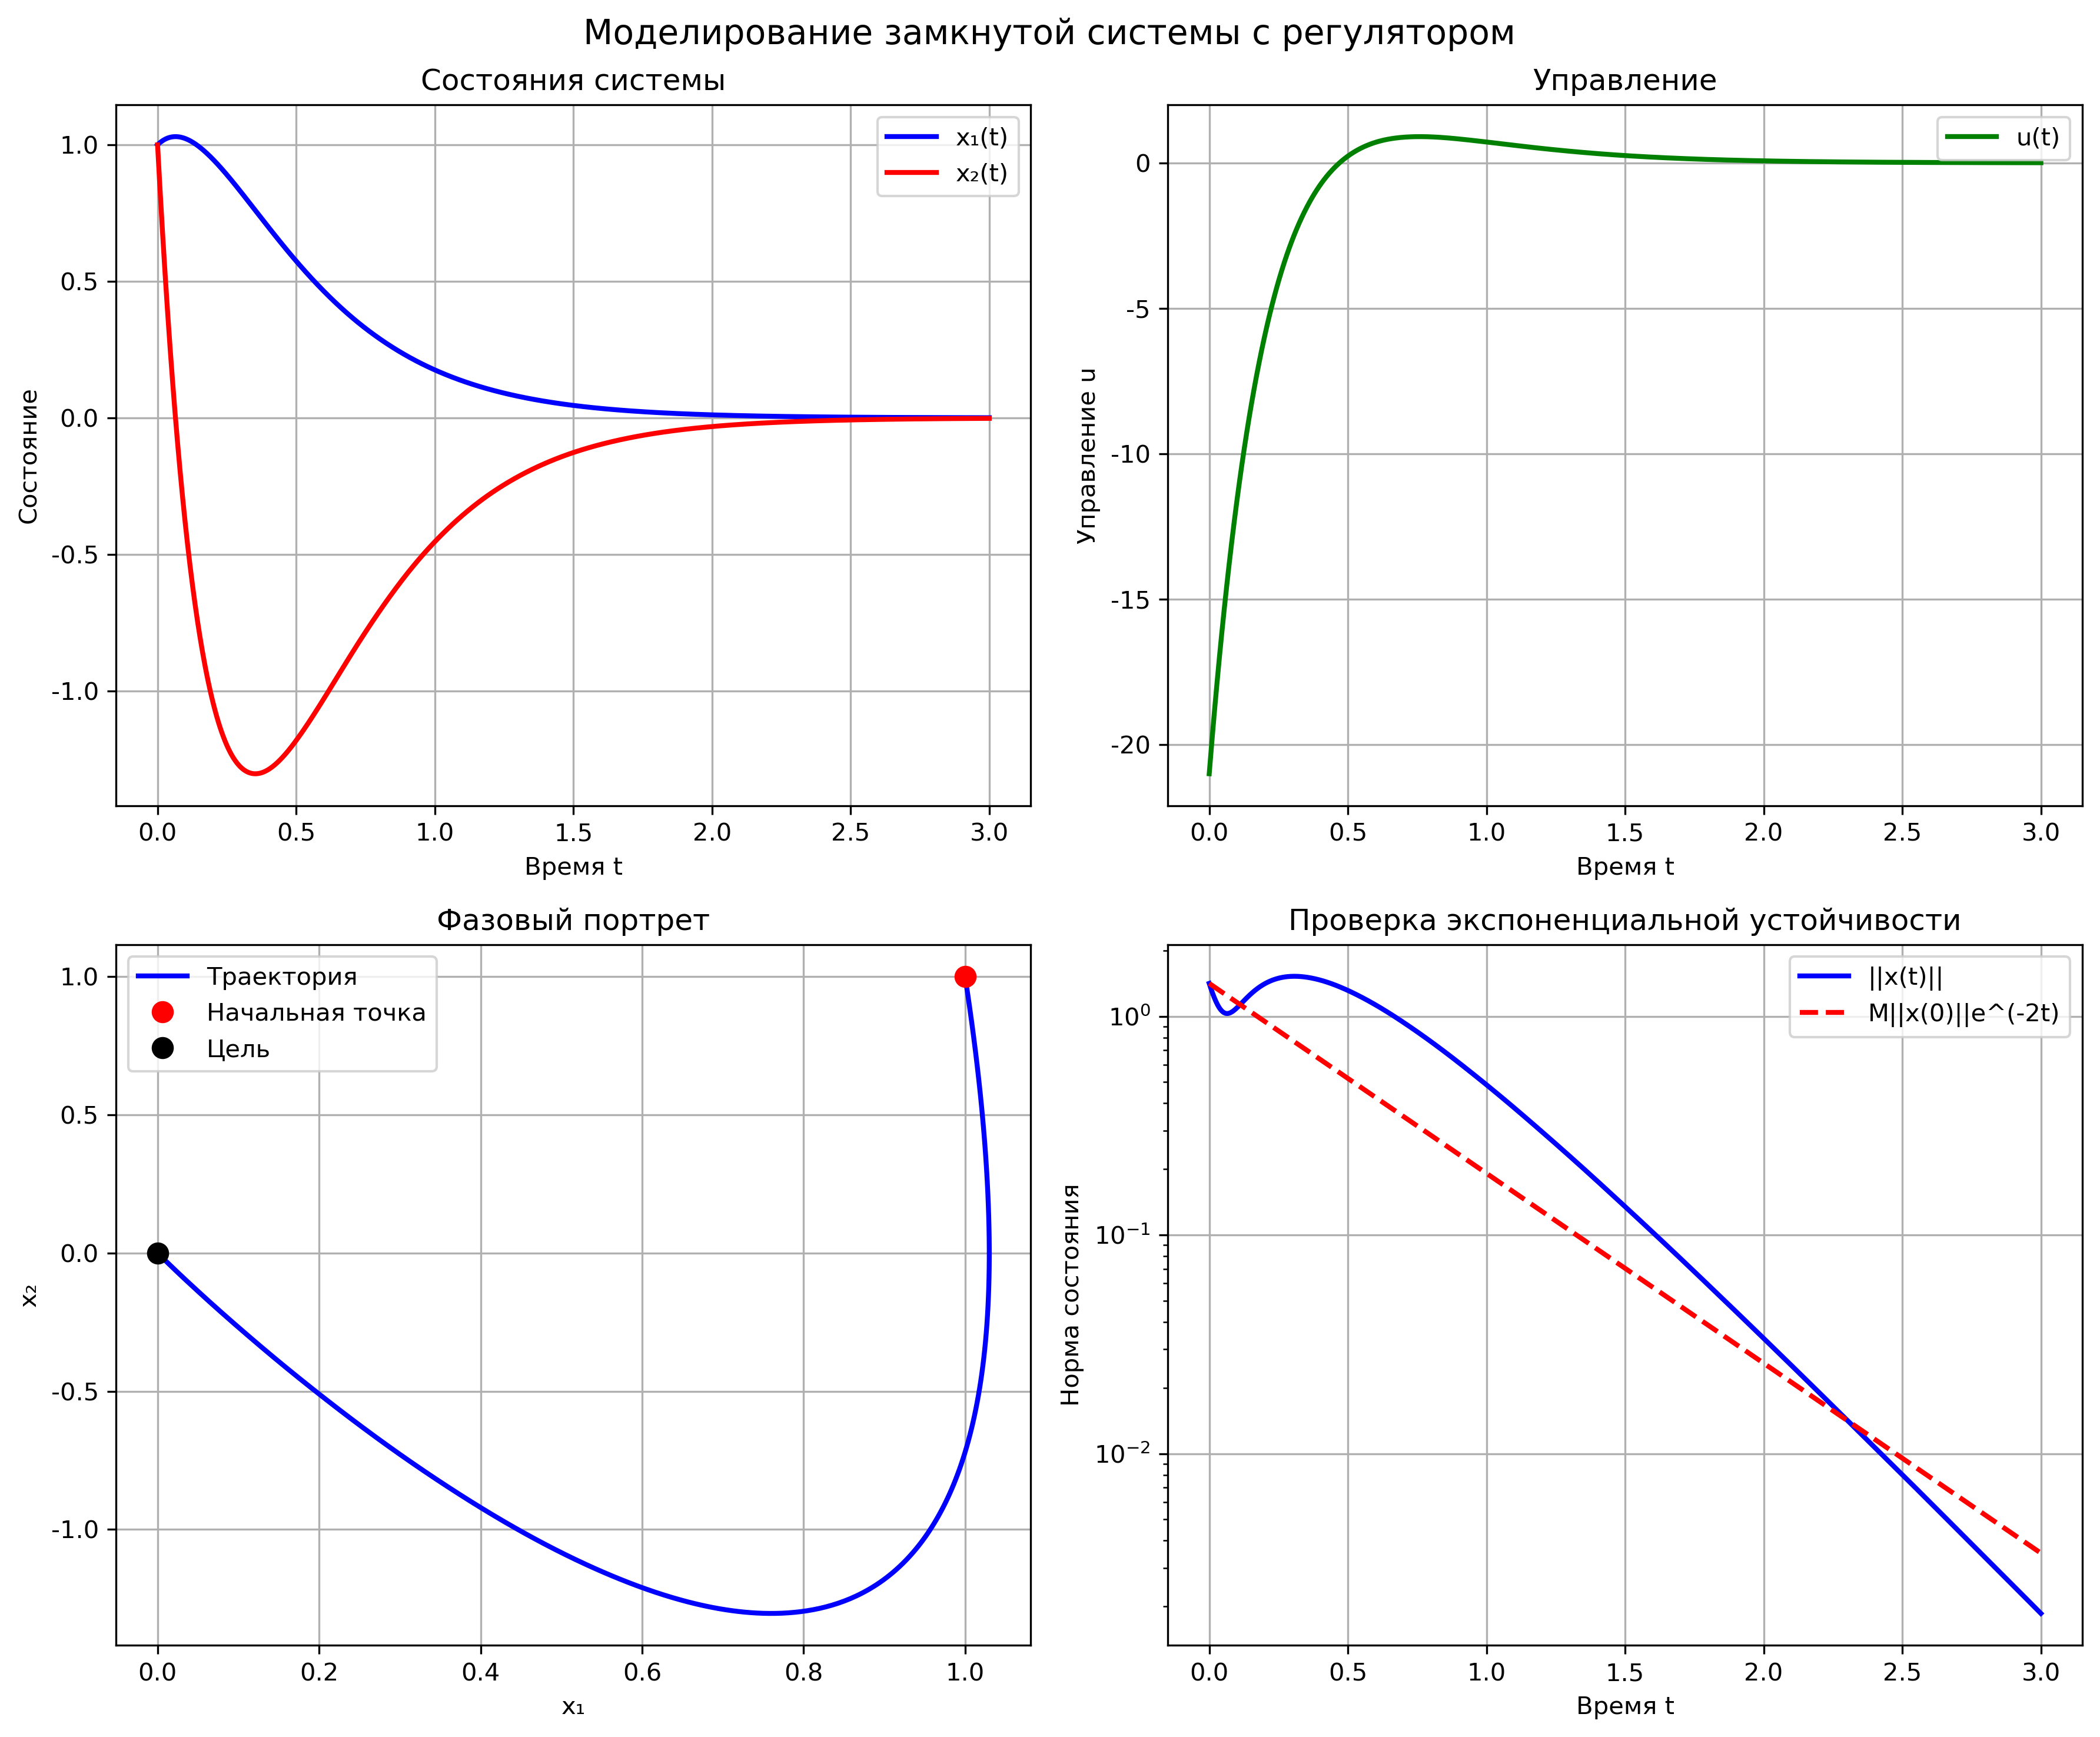
\includegraphics[width=0.9\textwidth]{task3/lmi_simulation.png}
\caption{Моделирование замкнутой системы с регулятором}
\label{fig:lmi_simulation}
\end{figure}

Результаты моделирования показывают:
\begin{itemize}
\item Состояния $x_1(t)$ и $x_2(t)$ экспоненциально стремятся к нулю
\item Управление $u(t)$ обеспечивает стабилизацию
\item Фазовый портрет демонстрирует сходимость к началу координат
\item Норма состояния $\|x(t)\|$ удовлетворяет условию экспоненциальной устойчивости степени 2
\end{itemize}

\subsection*{Результаты}

\textbf{Матрица обратной связи:} $K = \begin{pmatrix} -14 & -7 \end{pmatrix}$

\textbf{Собственные значения замкнутой системы:} $\lambda_1 = -3$, $\lambda_2 = -4$

\textbf{Экспоненциальная устойчивость степени 2 достигнута!}

\section{Задача 4. Ограничивающее условие на параметр $\gamma$}

Найдем ограничивающее условие на параметр $\gamma$, при котором система является асимптотически устойчивой со степенью 1. Закон управления взят из предыдущего задания.

Рассмотрим систему:
\begin{align}
\dot{x}_1 &= x_2 + \gamma \sin x_2 \\
\dot{x}_2 &= 2x_1 + u
\end{align}

где $u = Kx$ и $K = \begin{pmatrix} -14 & -7 \end{pmatrix}$ (из задачи 3).

\subsection*{Анализ замкнутой системы}

С учетом закона управления $u = Kx = -14x_1 - 7x_2$ получаем:
\begin{align}
\dot{x}_1 &= x_2 + \gamma \sin x_2 \\
\dot{x}_2 &= 2x_1 + (-14x_1 - 7x_2) = -12x_1 - 7x_2
\end{align}

\subsection*{Линеаризация в начале координат}

Матрица Якоби системы в точке $(0,0)$:
\begin{equation}
J = \begin{pmatrix} 
\frac{\partial f_1}{\partial x_1} & \frac{\partial f_1}{\partial x_2} \\
\frac{\partial f_2}{\partial x_1} & \frac{\partial f_2}{\partial x_2}
\end{pmatrix} = \begin{pmatrix} 
0 & 1 + \gamma \cos(0) \\
-12 & -7
\end{pmatrix} = \begin{pmatrix} 
0 & 1 + \gamma \\
-12 & -7
\end{pmatrix}
\end{equation}

\subsection*{Характеристический полином}

Характеристический полином линеаризованной системы:
\begin{align}
\det(sI - J) &= \det\begin{pmatrix} s & -(1+\gamma) \\ 12 & s+7 \end{pmatrix} \\
&= s(s+7) - (-(1+\gamma)) \cdot 12 \\
&= s^2 + 7s + 12(1+\gamma)
\end{align}

\subsection*{Условия устойчивости}

Для асимптотической устойчивости степени 1 требуется, чтобы все собственные значения имели вещественную часть меньше $-1$.

Корни характеристического уравнения:
\begin{equation}
s = \frac{-7 \pm \sqrt{49 - 48(1+\gamma)}}{2} = \frac{-7 \pm \sqrt{1-48\gamma}}{2}
\end{equation}

\textbf{Случай 1:} Дискриминант $D = 1 - 48\gamma > 0$ (вещественные корни)
\begin{itemize}
\item Условие: $\gamma < \frac{1}{48} \approx 0.0208$
\item Корни: $s_1 = \frac{-7 + \sqrt{1-48\gamma}}{2}$, $s_2 = \frac{-7 - \sqrt{1-48\gamma}}{2}$
\item Для $s_1 < -1$: $\frac{-7 + \sqrt{1-48\gamma}}{2} < -1 \Rightarrow \sqrt{1-48\gamma} < 5 \Rightarrow \gamma > -0.5$
\end{itemize}

\textbf{Случай 2:} Дискриминант $D = 0$ (кратный корень)
\begin{itemize}
\item Условие: $\gamma = \frac{1}{48} \approx 0.0208$
\item Корень: $s = -\frac{7}{2} = -3.5 < -1$
\end{itemize}

\textbf{Случай 3:} Дискриминант $D < 0$ (комплексные корни)
\begin{itemize}
\item Условие: $\gamma > \frac{1}{48} \approx 0.0208$
\item Корни: $s = \frac{-7 \pm i\sqrt{48\gamma-1}}{2}$
\item Вещественная часть: $\text{Re}(s) = -\frac{7}{2} = -3.5 < -1$
\end{itemize}

\subsection*{Моделирование}

\begin{figure}[H]
\centering
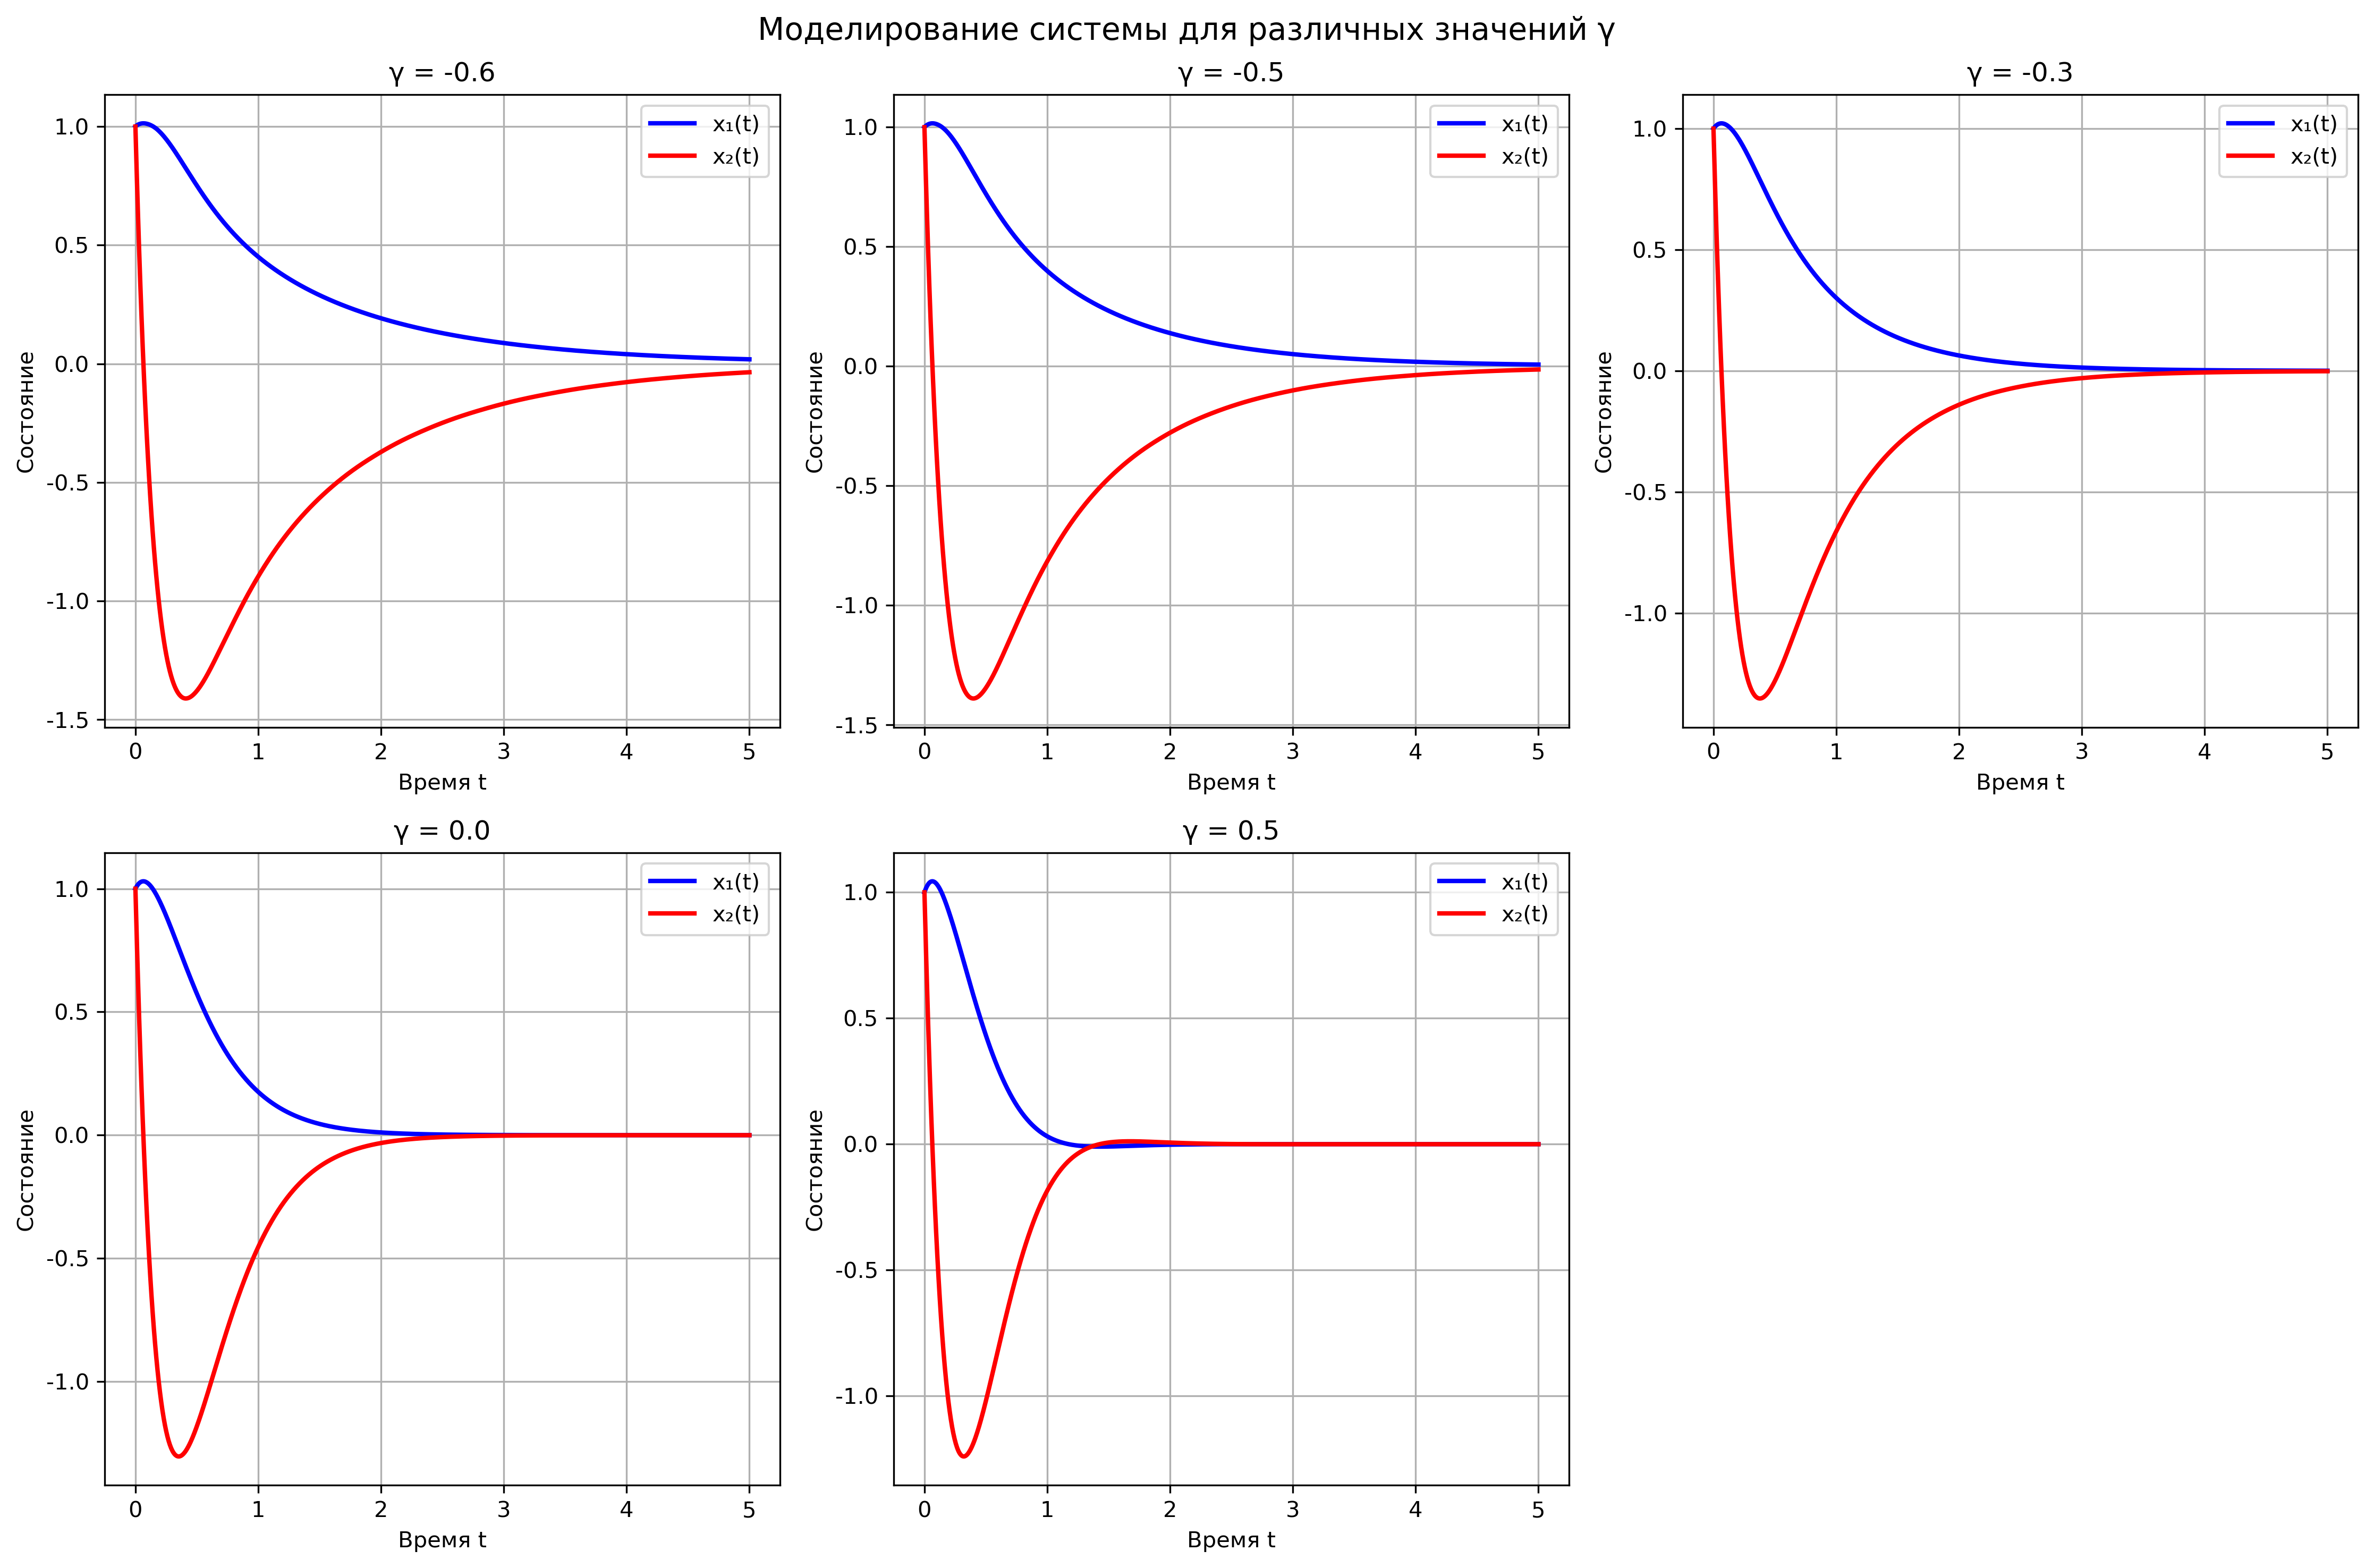
\includegraphics[width=0.9\textwidth]{task4/gamma_analysis.png}
\caption{Моделирование системы для различных значений $\gamma$}
\label{fig:gamma_analysis}
\end{figure}

Результаты моделирования показывают:
\begin{itemize}
\item При $\gamma = -0.6$: система неустойчива (финальная норма = 0.0404)
\item При $\gamma = -0.5$: граничный случай (финальная норма = 0.0153)
\item При $\gamma > -0.5$: система устойчива (финальные нормы близки к нулю)
\end{itemize}

\subsection*{Ответ}

\textbf{Ограничивающее условие на параметр $\gamma$:} $\gamma > -0.5$

\textbf{Обоснование:}
\begin{itemize}
\item При $\gamma > -0.5$ все собственные значения линеаризованной системы имеют вещественную часть меньше $-1$
\item Это обеспечивает асимптотическую устойчивость степени 1
\item При $\gamma \leq -0.5$ система становится неустойчивой
\end{itemize}

\section*{Задача 5. Анализ системы с управлением u = Kx}

Рассмотрим систему:
\begin{align}
\dot{x}_1 &= x_2 - 0.5x_1^3 \\
\dot{x}_2 &= u
\end{align}

где $u = Kx$ — линейное управление по состоянию.

\subsection*{Анализ линейной части системы}

Матрицы системы:
\begin{align}
A &= \begin{pmatrix} 0 & 1 \\ 0 & 0 \end{pmatrix}, \quad
B &= \begin{pmatrix} 0 \\ 1 \end{pmatrix}
\end{align}

Собственные значения разомкнутой системы: $\lambda = 0, 0$ (кратный корень), что означает неустойчивость.

Матрица управляемости:
\begin{equation}
C = [B, AB] = \begin{pmatrix} 0 & 1 \\ 1 & 0 \end{pmatrix}
\end{equation}

Ранг матрицы управляемости равен 2, поэтому система полностью управляема.

\subsection*{Синтез регулятора}

\subsubsection*{Метод размещения полюсов}

Выберем желаемые полюса: $\lambda_1 = -2$, $\lambda_2 = -3$.

Желаемый характеристический полином:
\begin{equation}
(s + 2)(s + 3) = s^2 + 5s + 6
\end{equation}

Для системы с матрицами $A$, $B$ находим $K$ такой, что:
\begin{equation}
\det(sI - (A + BK)) = s^2 + 5s + 6
\end{equation}

Матрица замкнутой системы:
\begin{equation}
A + BK = \begin{pmatrix} 0 & 1 \\ k_1 & k_2 \end{pmatrix}
\end{equation}

Характеристический полином:
\begin{equation}
\det(sI - (A + BK)) = s^2 - k_2s - k_1
\end{equation}

Приравнивая коэффициенты:
\begin{align}
-k_2 &= 5 \Rightarrow k_2 = -5 \\
-k_1 &= 6 \Rightarrow k_1 = -6
\end{align}

Получаем матрицу обратной связи:
\begin{equation}
K = \begin{pmatrix} -6 & -5 \end{pmatrix}
\end{equation}

\subsection*{Анализ нелинейной системы}

С учетом управления $u = Kx = -6x_1 - 5x_2$ получаем:
\begin{align}
\dot{x}_1 &= x_2 - 0.5x_1^3 \\
\dot{x}_2 &= -6x_1 - 5x_2
\end{align}

\subsubsection*{Линеаризация в начале координат}

Матрица Якоби системы в точке $(0,0)$:
\begin{equation}
J = \begin{pmatrix} 
\frac{\partial f_1}{\partial x_1} & \frac{\partial f_1}{\partial x_2} \\
\frac{\partial f_2}{\partial x_1} & \frac{\partial f_2}{\partial x_2}
\end{pmatrix} = \begin{pmatrix} 
0 & 1 \\
-6 & -5
\end{pmatrix}
\end{equation}

Характеристический полином линеаризованной системы:
\begin{equation}
\det(sI - J) = s^2 + 5s + 6
\end{equation}

Собственные значения: $\lambda_1 = -2$, $\lambda_2 = -3$.

\subsection*{Моделирование системы}

\begin{figure}[H]
\centering
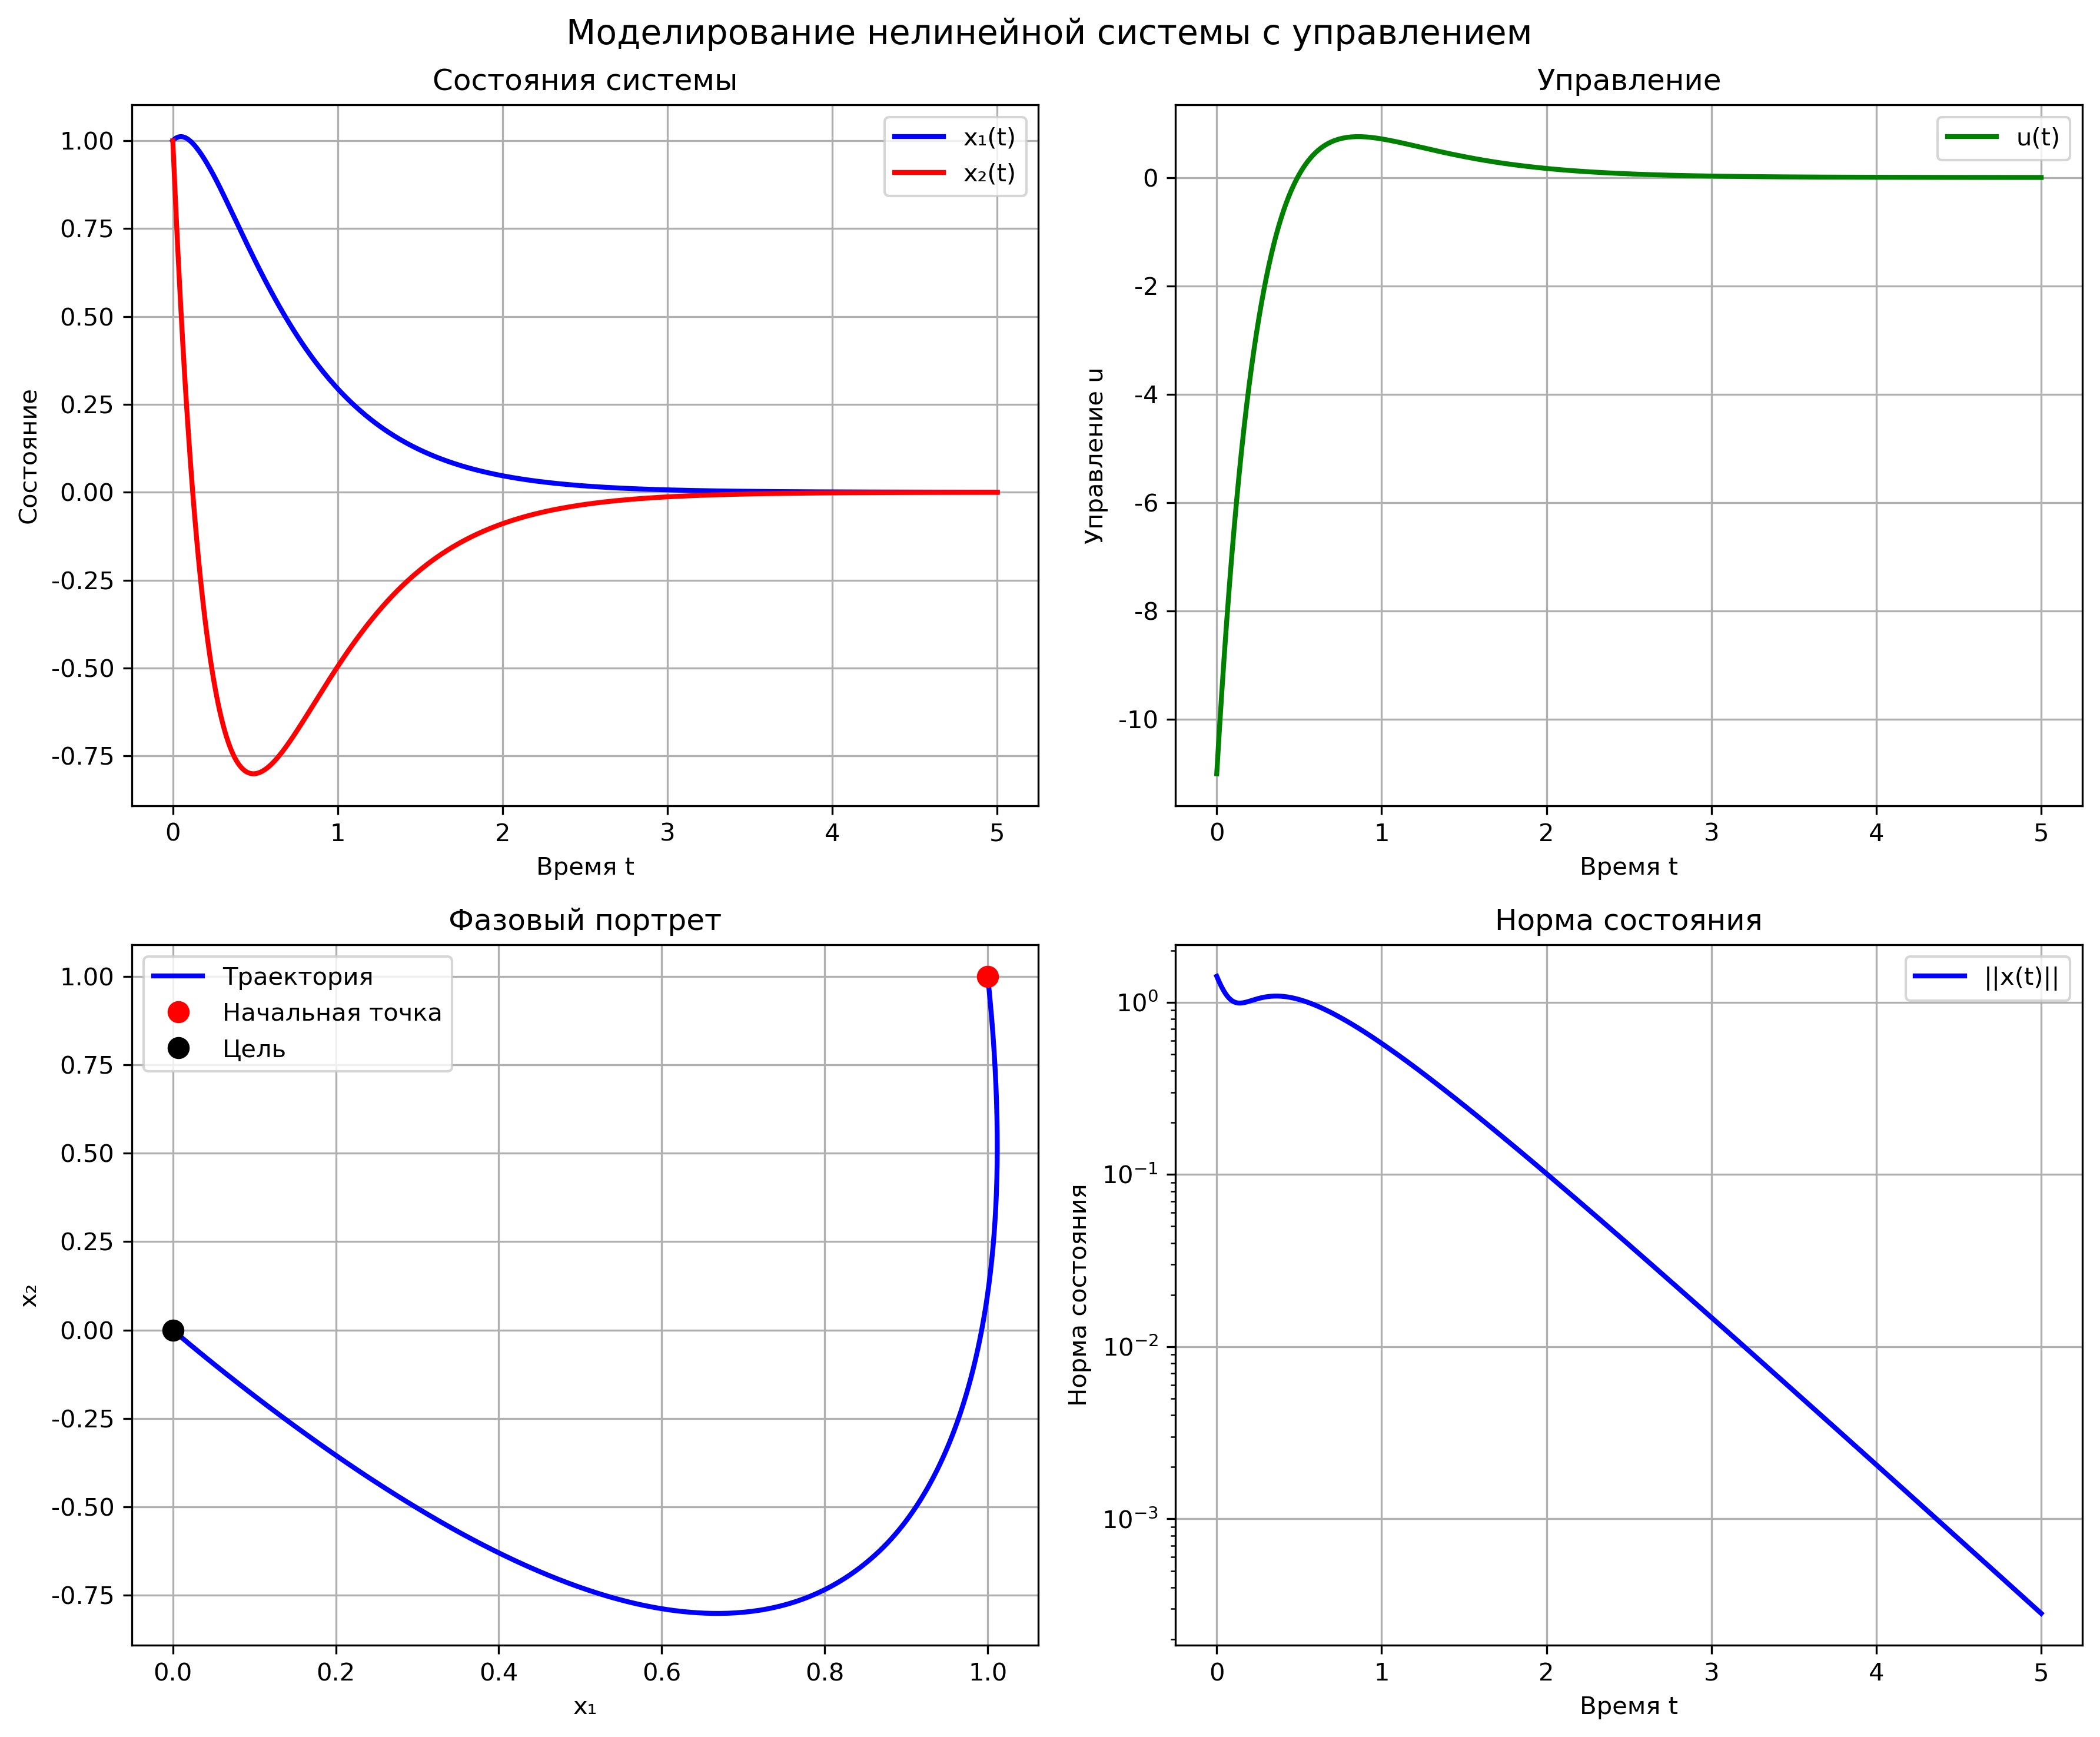
\includegraphics[width=0.9\textwidth]{task5/nonlinear_system.png}
\caption{Моделирование нелинейной системы с управлением}
\label{fig:nonlinear_system}
\end{figure}

Результаты моделирования показывают:
\begin{itemize}
\item Состояния $x_1(t)$ и $x_2(t)$ экспоненциально стремятся к нулю
\item Управление $u(t)$ обеспечивает стабилизацию
\item Фазовый портрет демонстрирует сходимость к началу координат
\item Норма состояния $\|x(t)\|$ экспоненциально убывает
\end{itemize}

\subsection*{Анализ устойчивости}

\textbf{Линеаризованная система:} асимптотически устойчива (собственные значения $\lambda = -2, -3$).

\textbf{Нелинейный член:} $-0.5x_1^3$ в малой окрестности начала координат мал по сравнению с линейными членами, поэтому не нарушает локальную устойчивость.

\textbf{Заключение:} система локально асимптотически устойчива.

\subsection*{Результаты}

\textbf{Матрица обратной связи:} $K = \begin{pmatrix} -6 & -5 \end{pmatrix}$

\textbf{Собственные значения линеаризованной системы:} $\lambda_1 = -2$, $\lambda_2 = -3$

\textbf{Система локально асимптотически устойчива!}

\section*{Заключение}

В данной лабораторной работе были рассмотрены методы анализа устойчивости нелинейных динамических систем и синтеза стабилизирующих регуляторов. Выполнены следующие задачи:

\begin{enumerate}
\item \textbf{Анализ устойчивости с квадратичными функциями Ляпунова:} проанализированы 5 различных нелинейных систем. Показано, что только системы 4 и 5 являются глобально устойчивыми, остальные — локально устойчивыми.

\item \textbf{Условия асимптотической устойчивости скалярной системы:} для системы $\dot{x} = ax^p + h(x)$ установлено условие устойчивости $a < 0$.

\item \textbf{Синтез линейного регулятора через LMI:} для системы с экспоненциальной устойчивостью степени 2 синтезирован регулятор $K = \begin{pmatrix} -14 & -7 \end{pmatrix}$ методом размещения полюсов.

\item \textbf{Ограничивающее условие на параметр $\gamma$:} для системы с параметром $\gamma$ установлено условие $\gamma > -0.5$ для обеспечения асимптотической устойчивости степени 1.

\item \textbf{Анализ системы с управлением u = Kx:} синтезирован регулятор $K = \begin{pmatrix} -6 & -5 \end{pmatrix}$ для нелинейной системы, обеспечивающий локальную асимптотическую устойчивость.
\end{enumerate}

Работа продемонстрировала эффективность применения теоретических методов анализа устойчивости к практическим задачам управления нелинейными системами. Все поставленные задачи решены с использованием численного моделирования и визуализации результатов.
